\documentclass{article}%
\usepackage[T1]{fontenc}%
\usepackage[utf8]{inputenc}%
\usepackage{lmodern}%
\usepackage{textcomp}%
\usepackage{lastpage}%
\usepackage[head=40pt,margin=0.5in,bottom=0.6in]{geometry}%
\usepackage{graphicx}%
%
\title{\textbf{La venezolana Susana Raffalli fue premiada por su labor en derechos humanos}}%
\author{EFE}%
\date{21/11/2018}%
%
\begin{document}%
\normalsize%
\maketitle%
\textbf{URL: }%
http://www.el{-}nacional.com/noticias/mundo/venezolana{-}susana{-}raffalli{-}fue{-}premiada{-}por{-}labor{-}derechos{-}humanos\_260569\newline%
%
\textbf{Periodico: }%
EN, %
ID: %
260569, %
Seccion: %
Mundo\newline%
%
\textbf{Palabras Claves: }%
Sociedad\newline%
%
\textbf{Derecho: }%
5%
, Otros Derechos: %
2.10%
, Sub Derechos: %
2.10.1%
\newline%
%
\textbf{EP: }%
NO\newline%
\newline%
%
\textbf{\textit{El chino Yu Wensheng, el indio Nityanand Jayaraman, la camboyana Chak Sopheap, la tailandesa Sirikan Charoensiri y el ruso Oyub Titiev son otros de los galardonados por los gobiernos de Alemania y Francia}}%
\newline%
\newline%
%
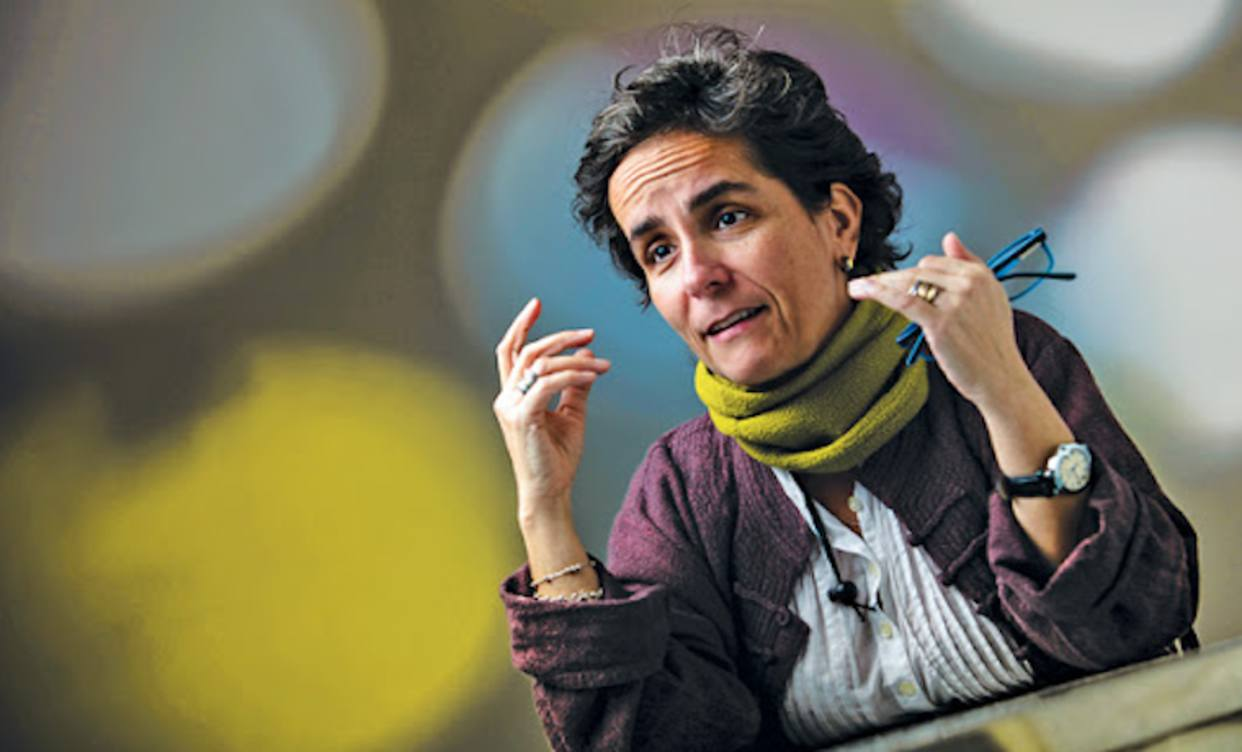
\includegraphics[width=300px]{165.jpg}%
\newline%
%
La venezolana~Susana~Raffalli~Arismendi y la peruana Liz Chicaje Churay y fueron galardonadas, junto a otras trece personas, con el premio Por los Derechos Humanos y el Estado de Derecho que entregan anualmente los gobiernos de Alemania y Francia.%
\newline%
%
Los ministros de Exteriores de Alemania y Francia, Heiko Maas y Jean{-}Yves Le Drian, anunciaron en un comunicado los nombres de los premiados, a los que homenajean porque "defienden valientemente la aplicación de los derechos humanos".%
\newline%
%
"Ellos representan también a los muchos defensores de los derechos humanos que permanecen en el anonimato por su tarea y que en su lucha por la justicia a menudo sufren grandes injusticias", se lee en el comunicado.%
\newline%
%
Francia y Alemania quisieron agradecer a los galardonados por "convertir en hechos" las palabras de la Declaración de los Derechos Humanos.%
\newline%
%
Entre los activistas reconocidos por este premio destacan los procedentes de África y Oriente Medio, como Mohamed Lotfy (Egipto), Alfredo Okenve (Guinea Ecuatorial), Aminata Traoré (Costa de Marfil), Hessen Sayah Corban (Líbano), Memo Mekfoula Mint Brahim (Mauritania), Daoud Nassar (Palestina), Vuyiseka Dubula{-}Majola (Suráfrica) y Anwar al{-}Bunni (Siria).%
\newline%
%
Asimismo, han sido premiados por su labor el chino Yu Wensheng, el indio Nityanand Jayaraman, la camboyana Chak Sopheap, la tailandesa Sirikan Charoensiri y el ruso Oyub Titiev.%
\newline%
%
Alemania y Francia conceden este año por tercera vez este galardón, que busca premiar a "personalidades de todo el mundo" que defienden "la protección y la promoción de los derechos humanos".%
\newline%
%
Ambos países buscan con este premio demostrar su compromiso con la cooperación común~en el ámbito de los derechos humanos.%
\newline%
%
\end{document}